% Technical report (English, draft). Build: bash docs/report/build.sh
\documentclass[10pt,a4paper,twocolumn]{article}
\usepackage[margin=17mm,columnsep=6mm]{geometry}
\usepackage{amsmath,amssymb}
\usepackage{booktabs}
\usepackage{graphicx}
\usepackage{xcolor}
\usepackage{tikz}
\usetikzlibrary{positioning,arrows.meta,fit,calc}
\usepackage[font=small,labelfont=bf]{caption}
\usepackage{enumitem}
\setlist{nosep,leftmargin=*}
\usepackage{xeCJK}
\setCJKmainfont[Path=fonts/,BoldFont=NotoSerifJP-Bold.otf]{NotoSerifJP-Regular.otf}
\usepackage[colorlinks=true,linkcolor=blue!50!black,citecolor=blue!50!black,urlcolor=blue!50!black]{hyperref}
\newcommand{\pt}{\,pt}
\setlength{\emergencystretch}{1.5em}

\title{\bfseries A Physical Voice Model as the Decoder of a Speech Codec:\\
Encoders and Text-to-Speech on Its Control Tracks}
\author{Claude (Anthropic)\thanks{Claude (Fable 5.2), working in Claude Code, planned and implemented
the experiments, ran them, analyzed the results and wrote this report. Takuma Mori did the listening and gave the
overall direction.}\qquad Takuma Mori}
\date{{\small Technical report (draft), November 2026}\\
{\small\url{https://github.com/takuma104/physical-modeling-voice-codec}}}

\begin{document}
\maketitle

\begin{abstract}
A neural speech codec decodes any latent into sound, and when a model that predicts its latents
errs, the result can be a sound no vocal tract makes. We study a codec whose decoder cannot do
that: CHIMERA, an open-source physical model of the human voice (lungs, vocal folds, a branched
vocal tract), used without modification. The latent is its control track, 21 channels at 100\,Hz:
the positions of jaw, tongue, lips and velum, the state of the glottis, the breath and the pitch.
An encoder writes this track from a recording in one pass. It is taught without transcripts and
without searching for tracks, through a network that stands in for the simulator, which cannot be
differentiated. On English speakers it never heard, Whisper misreads 3.2\% of the words of its
renders (recordings: 1.6\%); on Japanese, 0.4\% of the phonemes (0.2\%). Noise on the track,
4-bit quantization and 25\,Hz sampling degrade the speech gradually, and to the ear the errors
are those of a person who articulates poorly. Two sounds that recordings do not have were traced
by listening to the simulator's own mechanics and removed through its public settings. A
text-to-speech model that writes the track from phonemes is read as well as the encoder (0.2\%
against 0.1\%). Taught with 200 sentences (15 minutes) of one speaker it gets 0.5\% of the
phonemes wrong, with 20 sentences (1.5 minutes) 7.7\%. A control says what of this the latent
does. The same model writing a mel spectrogram or EnCodec's latent is understood as well from
as little data, so that is the model's doing. The decoder shows in the sound when data is
scarce: with 20 and 200 sentences the physical model's predicted quality is 4.1 and 4.8, the
spectrogram's 2.6 and 3.5, and at best 3.2 and 4.1 once its vocoder is tuned on the model's
output. With 2,000 sentences the tuned vocoder reaches 4.5, where the recordings are. Taught with a hundred speakers it reads sentences it never
saw as intelligibly as their recordings are (2.3\% against 2.5\%). Of a speaker the codec
carries the sex and the pitch; with the simulator's body, glottis and habits of posture fitted
to each speaker, eleven more numbers, a verification model finds the speaker among eight for
57.0\% of the renders instead of 26.5\%, and among a hundred for 14.2\% instead of
2.8\% (recordings: 96.5\% and 93.7\%).
\end{abstract}

\section{Introduction}
Neural audio codecs~\cite{encodec,moshi} are the interface of today's speech generation: a language
or flow model predicts latents and a neural decoder turns them into a waveform. The decoder
accepts any latent. When the predictor is small or has seen little data, its errors come out as
whatever the decoder makes of an off-distribution latent: buzzing, metallic consonants, sounds
with no source in a mouth. One of us met this while adapting Pocket TTS, built on the Mimi codec,
to Japanese~\cite{pocketja}.

This report asks what happens if the decoder is a physical model of the voice. A simulator of
airflow through vocal folds and a vocal tract can only produce what such a system produces. If
its control parameters are the latent, an error in the latent is a tongue in the wrong place or a
glottis that closes late: a mistake of articulation, which is how people err too. The hypothesis
is that such a codec fails more gracefully, and that its latent, being close to what speech is
made of, is easy to predict from text.

Speech coding through articulation has a long history, and recent neural work encodes speech into
articulatory trajectories and decodes them with a neural vocoder: SPARC~\cite{sparc} (12
articulator coordinates, pitch and loudness at 50\,Hz, HiFi-GAN decoder) and
ARTI-6~\cite{arti6} (six features from real-time MRI). There the decoder is still a network.
Differentiable simulation of the tract~\cite{difftlm} recovers a tract shape from audio by
optimizing each utterance. Articulatory synthesizers such as VocalTractLab~\cite{vtl} are driven
by rules or by analysis-by-synthesis.

We take a physical synthesizer as it is, CHIMERA~\cite{chimera}, and build the rest around it:
\begin{itemize}
\item an \textbf{encoder} that writes the simulator's control track from a recording in one pass,
taught without transcripts through a learned stand-in for the simulator (\S\ref{sec:encoder});
\item evidence that \textbf{errors in the latent stay human}: noise, quantization and decimation
of the track (\S\ref{sec:perturb});
\item two \textbf{artifacts of the simulator} found by listening, traced to its mechanics and
removed through its settings, and settings for high voices (\S\ref{sec:voice});
\item a \textbf{text-to-speech model} on the latent that matches the encoder and learns from
minutes of speech (\S\ref{sec:tts});
\item a \textbf{control}: the same model on the latents of three neural decoders, which says
what the physical decoder contributes and what it does not (\S\ref{sec:control}).
\end{itemize}
Code is at the address above. The engine's code is unchanged throughout.

\section{The decoder and its latent}\label{sec:decoder}
\textbf{CHIMERA}~\cite{chimera} is a physical-modeling voice synthesizer written in Rust (MIT
license), made as an instrument for the browser. It simulates an airway in the time domain at
48\,kHz: a lung pressure, vocal folds whose area waveform drives a glottal port (the flow follows
from the pressure across it, so pulse skew and devoicing under a closed mouth come out of the
physics), a branched tract with nasal and lateral passages, radiation at lips, nose and walls,
and band-limited noise where the flow passes a constriction, the teeth or the glottis. A
\emph{body} parameter blends male, female and child tract sizes. Its own front end turns English
text into gestures by rule.

\textbf{The control track.} We bypass the front end. A small wrapper (PyO3) schedules one
frame of 21 control values every 10\,ms as targets for the engine's articulators and source
(Fig.~\ref{fig:channels}).
Besides the track the voice is told two things about a speaker: the sex, which picks the body,
and the median pitch. Speaker identity beyond that is not part of the latent
(\S\ref{sec:discussion}).

\begin{figure}[t]
\centering
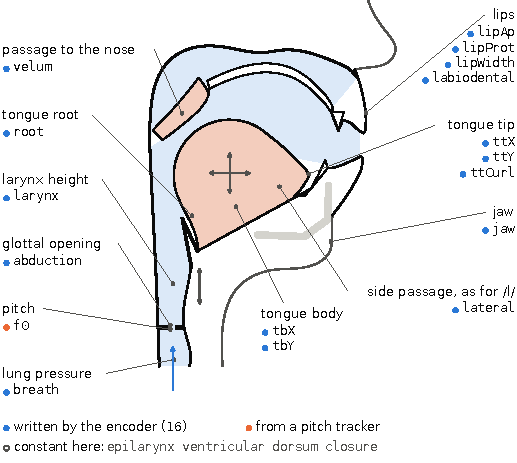
\includegraphics[width=\columnwidth]{fig_tract_en.pdf}
\caption{The decoder's vocal tract and the 21 channels of the control track (100\,Hz). The
outlines are CHIMERA's own, for its male body in a half-open vowel with the passage to the nose
open; what it simulates is the air between them (blue). Each channel is the target of one
articulator or of the voice source. The encoder writes the 16 that vary in speech, the pitch
comes from a pitch tracker, and four are held constant.}
\label{fig:channels}
\end{figure}

\textbf{Is the track enough?} Rendering CHIMERA's rule-made speech again from its own control
track at 100\,Hz changes little: the mel-cepstral distance to the original is 0.7\,dB and the
voicing agrees in 97\% of the frames. One CPU thread renders a 4\,s sentence in 0.5\,s.

\textbf{Data and judges.} English: the TSP speech database~\cite{tsp} (Harvard sentences read in an
anechoic room); four speakers (240 recordings) are held out for testing and two for validation,
with the sentence lists they read, leaving 1,012 recordings. Japanese: JVS~\cite{jvs} (100
speakers), Hi-Fi-CAPTAIN~\cite{hificaptain} (one woman, one man) and JSUT~\cite{jsut}. Every result
is judged by models that no training or tuning in this work optimizes: Whisper~\cite{whisper}
small (small.en for English) and large-v3-turbo, with greedy decoding, scored in words for English
and in phonemes of Open JTalk's~\cite{openjtalk} reading for Japanese; and a multilingual phone
recognizer~\cite{xlsrphone} that knows no text, which writes down a recording and its render in IPA
(\emph{phone mismatch}: the share of the recording's phones the render changes; another person
reading the same sentence scores 24--32\% on Japanese). Predicted quality is
NISQA~\cite{nisqa}, which is used to choose settings in two places (\S\ref{sec:voice},
\S\ref{sec:control}) and reported on other recordings. This is NISQA's model of speech quality;
its model of the naturalness of synthesized speech rates the simulator's voice lower, and is
reported in \S\ref{sec:control}.

\section{Encoders}\label{sec:encoder}
\begin{figure}[t]
\centering\footnotesize
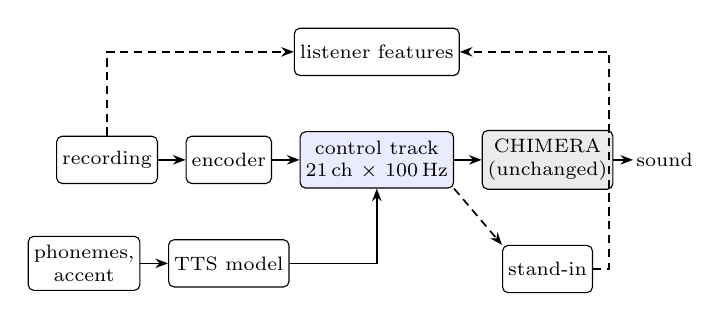
\begin{tikzpicture}[
  box/.style={draw, rounded corners=2pt, minimum height=6mm, inner xsep=2pt, align=center, font=\scriptsize},
  phys/.style={box, fill=black!8},
  arr/.style={-{Stealth[length=1.6mm]}, semithick},
  learn/.style={-{Stealth[length=1.6mm]}, semithick, densely dashed}]
\node[box] (rec) {recording};
\node[box, right=3.5mm of rec] (enc) {encoder};
\node[box, right=3.5mm of enc, fill=blue!8] (trk) {control track\\21\,ch $\times$ 100\,Hz};
\node[phys, right=3.5mm of trk] (sim) {CHIMERA\\(unchanged)};
\node[box, below=7mm of enc] (tts) {TTS model};
\node[box, left=3.5mm of tts] (txt) {phonemes,\\accent};
\node[box, below=7mm of sim] (std) {stand-in};
\node[box, above=7mm of trk] (lis) {listener features};
\draw[arr] (rec) -- (enc); \draw[arr] (enc) -- (trk); \draw[arr] (trk) -- (sim);
\draw[arr] (txt) -- (tts); \draw[arr] (tts) -| (trk);
\draw[learn] (trk.south east) -- (std.north west);
\draw[learn] (std.east) -- ++(2mm,0) |- (lis.east);
\draw[learn] (rec.north) |- (lis.west);
\node[right=2.5mm of sim, font=\scriptsize, inner sep=1pt] (out) {sound};
\draw[arr] (sim) -- (out);
\end{tikzpicture}
\caption{The codec. Solid: inference. Dashed: training. The stand-in predicts what a listener
model would hear of the track's render, so that the distance to what it hears in the recording
can be differentiated back into the encoder or the text-to-speech (TTS) model.}
\label{fig:system}
\end{figure}

\textbf{The network.} The encoder hears the recording through a self-supervised speech model (a
learned mix of its layers; in the later encoders the top six are tuned) and through three plain
features per frame: whether a pitch tracker~\cite{praat} calls the frame voiced, its pitch relative to the
speaker's median, and its level. Two bidirectional LSTM layers (width 256) write the 16 moving
channels at 100\,Hz. Pitch is not learned: the pitch channel is the tracker's contour. Encoding a
3\,s sentence takes about 0.08\,s.

\textbf{Three things to learn from} (Fig.~\ref{fig:system}, Table~\ref{tab:english}).
\emph{Renders.} CHIMERA's own speech gives exact pairs of sound and track without limit. An
encoder taught with them alone (A) already works on recordings, but no better than the rule
synthesis it learned from. \emph{Searched tracks.} A search that drives the simulator and
adjusts a track until a listener model finds the render close to the recording cuts A's word
errors from 34.6\% to 13.3\%, at one to two minutes per sentence. An encoder taught to copy such tracks (B) stalls: its
listener distance went from 0.18 to 0.17 when the tracks to copy grew from 170 to 1,012. Many
tracks make the same sound, and their average need not. \emph{The voice itself.} The remedy is
the distal teacher~\cite{distal}: teach the encoder through a model of what its output does.
CHIMERA is not differentiable, but its renders are free and exact, so a network (three
bidirectional LSTM layers, width 512) learns to map a track to what a listener would hear of its
render: the frame-level features of wav2vec\,2.0~\cite{wav2vec2}, later of
mHuBERT-147~\cite{mhubert}. The encoder's loss is then the distance (one minus cosine, frame
against frame) between what this \emph{stand-in} says of the track it wrote and what the listener
hears in the recording, plus a weak pull towards a reference track. The stand-in is crude, and
it suffices (C). The reference tracks need not be searched: A's own outputs serve (C$'$), which
removes the search from the recipe. Training takes 20--25 minutes on one GPU. The weights kept
are those of the epoch after which the simulator itself, driven by the encoder on validation
recordings, comes closest to them.

\begin{table}[t]
\centering\footnotesize\setlength{\tabcolsep}{3pt}
\caption{Encoders taught with English (TSP), on four held-out speakers (240 sentences). Word
error rate (\%) of Whisper small.en and large-v3-turbo; listener distance to the recording.}
\label{tab:english}
\begin{tabular}{@{}lrrr@{}}
\toprule
& small.en & large & Dist.\\
\midrule
Recordings & 2.6 & 1.6 & --\\
CHIMERA's rule synthesis from text & 36.2 & 25.5 & --\\
A: renders only & 34.6 & 31.0 & 0.28\\
Search from A's track (1--2 min/sentence) & 13.3 & 11.5 & 0.10\\
B: copies searched tracks & 19.5 & 15.1 & 0.19\\
C: B + stand-in loss & 6.5 & 5.2 & 0.11\\
C$'$: stand-in loss, no search & 7.9 & 6.0 & 0.13\\
\bottomrule
\end{tabular}
\end{table}

The search reaches the smallest distance and yet reads worse than C: it fits each sentence to the
listener, while the encoder has to find what all sentences share. The encoder's articulators also
move more slowly than the rules' (the top 1\% of channel speeds is about 0.6 of theirs): it does
not win by shaking the tract in ways a recognizer likes.

\textbf{Japanese} (Table~\ref{tab:japanese}). C$'$, taught with English only, makes Japanese that
is understood but foreign: /o/ and /e/ come out as English vowels, and affricates and voiced
fricatives are lost (6--12\% of ざ-row consonants, じ, ち, つ and geminates). Three changes help,
and their gains add up: Japanese recordings in the closed loop (86 JVS speakers $\times$ 10
sentences, 1.9\,h, beside the English ones; D); a multilingual listener, mHuBERT-147 layer 8, in
place of the English wav2vec\,2.0 (E); both (F); and mHuBERT also as the encoder's front end (G).
The English listener had not been hearing the errors: it rated C$'$'s Japanese closer to the
recording than another person's reading of the sentence, while mHuBERT and the phone recognizer
rate it farther. With G the phone mismatch equals that of another real speaker, and English
improves as well.

\begin{table}[t]
\centering\footnotesize\setlength{\tabcolsep}{2.6pt}
\caption{Encoders on speakers and sentences they never heard. JVS: 8 speakers $\times$ 25
sentences; HFC+JSUT: Hi-Fi-CAPTAIN's two Japanese speakers and JSUT, 300 sentences; TSP: as in
Table~\ref{tab:english}. Whisper large-v3-turbo errors (\%, phonemes for Japanese, words for
English) and phone mismatch (\%). I is played by the voice of \S\ref{sec:voice}, the others by
CHIMERA's default.}
\label{tab:japanese}
\begin{tabular}{@{}lrrrrrr@{}}
\toprule
& \multicolumn{2}{c}{JVS} & \multicolumn{2}{c}{HFC+JSUT} & \multicolumn{2}{c}{TSP (en)}\\
& err. & phone & err. & phone & err. & phone\\
\midrule
Recordings & 2.5 & -- & 0.2 & -- & 1.6 & --\\
Another speaker & -- & 32.1 & -- & 24.1 & -- & 8.9\\
C$'$ (English only) & 6.6 & 42.6 & 2.9 & 40.8 & 6.0 & 10.9\\
G (+ Japanese, mHuBERT) & 3.9 & 28.0 & 0.4 & 26.6 & 3.5 & 8.5\\
H (+ silences) & 3.6 & 28.3 & 0.5 & 26.8 & 3.9 & 8.9\\
I (for the settled voice) & 3.4 & 29.3 & 0.4 & 27.3 & 3.2 & 9.4\\
\bottomrule
\end{tabular}
\end{table}

\textbf{Silence.} G voiced a sound before the speech in 51\% of the JVS recordings. The closed
loop compares only where the recording has speech; outside it the reference track was A's output,
and A starts to breathe as soon as it hears the room. In H the reference has no breath outside
the speech, and the stray sounds are gone (0\%) at the same intelligibility.

\section{Errors in the latent}\label{sec:perturb}
The hypothesis is about what errors sound like. We perturb the tracks that C$'$ writes for 40 test
sentences and render them (Table~\ref{tab:perturb}). The simulator never diverged or produced an
over-loud sound under any condition. Noise at a tenth of each channel's movement (20\,dB) leaves the
word error rate where it was; at a third (10\,dB) the speech becomes hard to follow. Four bits per channel or half
the frame rate cost little, so a naive code of 17 channels (the 16 and the pitch) $\times$
50\,Hz $\times$ 5\,bits, 4.2\,kbit/s with no entropy coding, reads as well as the unquantized
track.

\begin{table}[t]
\centering\footnotesize\setlength{\tabcolsep}{2pt}
\caption{Perturbing encoder C$'$'s tracks (40 sentences of the test speakers). Word error rate
of Whisper small.en (\%), with 95\% bootstrap intervals for the two references. Noise levels
are signal-to-noise ratios against how far each channel moves in speech; smooth noise varies
below 4\,Hz, an error that drifts.}
\label{tab:perturb}
\begin{tabular}{@{}lr@{\hspace{7pt}}lr@{}}
\toprule
\multicolumn{2}{@{}l}{Unperturbed: 5.2 [2.7, 8.1]} & \multicolumn{2}{l}{Recordings: 1.9 [0.6, 3.8]}\\
\midrule
White noise, 20\,dB & 6.2 & Quantized, 5 bits & 4.9\\
\quad 10\,dB & 17.0 & \quad 4 bits & 6.5\\
\quad 5\,dB & 34.0 & \quad 3 bits & 10.8\\
Smooth noise, 20\,dB & 6.2 & \quad 2 bits & 27.8\\
\quad 10\,dB & 26.2 & Sampled at 50\,Hz & 5.6\\
\quad 5\,dB & 68.5 & \quad 25\,Hz & 9.6\\
50\,Hz, 5 bits (4.2\,kb/s) & 5.2 & \quad 12.5\,Hz & 50.0\\
50\,Hz, 4 bits (3.4\,kb/s) & 8.0 & 25\,Hz, 4 bits (1.7) & 10.8\\
\bottomrule
\end{tabular}
\end{table}

What the numbers cannot say is how the failures sound. To the listener among us, the perturbed
renders sound ``like a person with poor articulation'', not like the artifacts of a codec; even
white noise on the controls, the most artificial condition, is not grating. The same holds for a
text-to-speech model that has seen too little data (\S\ref{sec:tts}).

\section{The voice}\label{sec:voice}
The simulator's fixed settings matter little for intelligibility, but three properties of its
sound did not survive listening. Each was traced to a mechanism and changed through settings the
engine exposes; the engine's code stayed as it is.

\textbf{High voices.} The male renders sounded real and the female ones thin. NISQA agrees: male
renders score like recordings (4.6--4.9), female ones 2.8--3.3. Over 17 speakers the score follows
the speaker's median pitch (correlation $-0.9$), whatever the sex, and lowering the pitch of a
woman's track by an octave restores it (2.9 to 4.4). The cause is the glottis: the engine's open
quotient is about 0.6 at every pitch, where real high voices open longer. Setting it to 0.85
directly, with a vibration amplitude of 1.4 and the source's tension, brightness and roughness
lowered, fitted on 16 sentences of one woman, raises the women of all three tests (Table~\ref{tab:voice}).
The settings harm low voices, so a speaker gets them in proportion to the median pitch: not at
all up to 150\,Hz, fully from 175\,Hz. Fitting to NISQA alone finds loopholes (louder noise
sources, which mask rather than mend), and the final values were set by ear.

\textbf{Sounds inside silences.} With the high voice fixed, a wet, tongue-smacking sound remained.
Muting stretches of a render in an audio editor showed that it lived in unvoiced stretches. One
part of it is air: CHIMERA lets the air that moving walls displace flow into the tract, so a
track played with no breath at all is not silent but thumps below a few hundred hertz, some
40\,dB under the speech (30\,dB for the male body), where a recording's closures and pauses are
silent. The engine has a switch for this flow, and the encoder's tracks are given no breath in
the recording's pauses.

\textbf{The click of a closure.} The smacking survived that. It was finally located in six
stretches of about 35\,ms next to voiced sound, above 2\,kHz, in one sentence. There, as the tongue
closes for a stop, the render has a click of one or two milliseconds that reaches 16\,kHz, 25--35\,dB
under the speech, where the recording has nothing. Turning off every noise source changes it by
less than 0.1\,dB: it is not turbulence. Tracing the engine's state sample by sample showed that
it treats a constriction below $2\cdot10^{-4}$\,cm$^2$ as closed and sets the flow through it to
zero within one sample, while about 1\,cm$^3$/s is still flowing. With the threshold at
$10^{-6}$\,cm$^2$ the flow has died away by itself. Our first two measures had missed the click
(one looked only below 9\,kHz and for bursts that stand out of the 20\,ms before them, the other
skipped the first 15\,ms of a silence); the one that found it assumes nothing about place or
shape and counts, band by band, what a render has that its recording has not.

\begin{table}[t]
\centering\scriptsize\setlength{\tabcolsep}{1.7pt}
\caption{The voice on the Japanese test recordings of women (JVS: 100; Hi-Fi-CAPTAIN and
JSUT: 200). NISQA; how often per second of speech the render sounds inside the recording's
silences (S) and clicks as a closure sets in (C); phone mismatch (\%). Rows 2--4 play encoder
H's tracks.}
\label{tab:voice}
\begin{tabular}{@{}lrrrrrrrr@{}}
\toprule
& \multicolumn{4}{c}{JVS} & \multicolumn{4}{c}{HFC+JSUT}\\
& NISQA & S & C & ph. & NISQA & S & C & ph.\\
\midrule
Recordings & 4.80 & -- & -- & -- & 4.57 & -- & -- & --\\
Default voice & 3.02 & .57 & .71 & 30.1 & 3.32 & .55 & 1.27 & 28.1\\
+ wall air off, closed area & 2.95 & .03 & .11 & 30.8 & 3.38 & .03 & .23 & 29.1\\
+ high-voice settings & 3.84 & .06 & .25 & 33.1 & 4.09 & .05 & .40 & 31.2\\
Encoder I, same voice & 3.91 & .02 & .28 & 31.3 & 4.10 & .03 & .44 & 28.9\\
\bottomrule
\end{tabular}
\end{table}

\textbf{An encoder for the voice.} H was taught through a stand-in for the default voice, and
under the new one it confuses voiced and voiceless stops more often (278 against 141 confusions in
500 Japanese sentences). Rendering the 3,864 training tracks again under the settled voice,
teaching a new stand-in from them and the encoder through it (I; 32 minutes in all) brings the
confusions down to 200 and the phone mismatch most of the way back, with the sound unchanged
(Tables~\ref{tab:japanese} and~\ref{tab:voice}).

\textbf{What remains.} The bursts when a stop is released are sharper than in recordings: at the
speaker's releases the render is as strong as the recording above 4\,kHz but 5--7\,dB weaker
below. Opening speed, lung pressure, breath during the closure, abduction and noise gains were
tried and none brings them closer without a side effect.

\section{Text-to-speech on the latent}\label{sec:tts}
\textbf{Model.} A sentence is read by Open JTalk~\cite{openjtalk} into phonemes; each carries
where its mora stands in its accent phrase (how far from the accent nucleus, how far from the
phrase's start and end) and whether the sentence asks. The model has the shape of
FastSpeech\,2~\cite{fastspeech2}: four self-attention blocks over the phonemes, a predictor of
each phoneme's duration, and six blocks over the frames that write the track: the 16 channels
and the pitch, which the encoder took from a tracker and which is written here too (width 256,
18.8M weights). Durations for training come from an alignment learned from the recordings and
their phonemes alone~\cite{ota}, with no external aligner.

\textbf{Data and losses.} The targets are encoder I's tracks for 18,655 sentences (24 hours) of
Hi-Fi-CAPTAIN's Japanese man; the 100 sentences of the corpus's evaluation set are the test. The
loss is the error against those tracks, the error of the log durations, and the encoder's
stand-in loss against the recording (Fig.~\ref{fig:system}). Two corrections make the timing the
speaker's. Log durations are short of the speaker's in sum, so they are scaled by a constant
(1.02). And the speaker pauses where the text has no comma, about 0.4 times per sentence for a
third of a second: the aligner marks such pauses, which would otherwise make a 390\,ms /d/, and
a small classifier on the model's states at accent-phrase borders decides where to pause at
inference (it places 27 pauses where the speaker makes 44 in the test sentences).

\begin{table}[t]
\centering\footnotesize\setlength{\tabcolsep}{2.2pt}
\caption{Text-to-speech on the 100 test sentences. Whisper errors (\% of phonemes), phone
mismatch (\%), NISQA; listener distance and pitch correlation with the recording, where the
render shares its timing.}
\label{tab:tts}
\begin{tabular}{@{}lrrrrrr@{}}
\toprule
& small & large & phone & NISQA & dist. & $r_{F0}$\\
\midrule
Recordings & 0.5 & 0.1 & -- & 4.56 & -- & --\\
Encoder I (from audio) & 1.3 & 0.1 & 24.2 & 4.75 & 0.192 & 0.99\\
TTS, speaker's timing & 0.7 & 0.1 & 24.6 & 4.80 & 0.207 & 0.92\\
TTS, from text alone & 0.8 & 0.2 & 24.7 & 4.78 & -- & --\\
\bottomrule
\end{tabular}
\end{table}

\textbf{Results} (Table~\ref{tab:tts}). From text alone the model's renders are read as well as
those of the encoder, which hears the recording, and score the same quality. The intonation is not
flattened: the pitch range is 97\% of the encoder's, and with the speaker's durations the pitch
correlates 0.92 with the recording's. On twelve sentences from outside the corpus large-v3-turbo
gets 0.4\% of the phonemes wrong; the one clear slip is /py/ (コンピューター comes out as
コンユーター), which occurs 35 times among the corpus's 951k phonemes. Writing the track for a 4\,s
sentence takes 17\,ms on a CPU.

\begin{figure}[t]
\centering
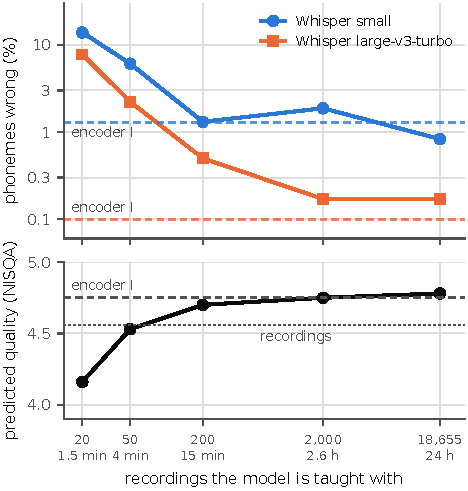
\includegraphics[width=\columnwidth]{fig_data_en.pdf}
\caption{The same text-to-speech model taught with fewer recordings of the speaker, on the 100
test sentences. Dashed: encoder I's renders of the recordings; dotted: the recordings.}
\label{fig:data}
\end{figure}

\textbf{Fewer recordings} (Fig.~\ref{fig:data}). The same model taught with 200 sentences, 15
minutes of speech, is still read almost without error (0.5\%), and with 20 sentences, a minute
and a half, large-v3-turbo still gets 92\% of the phonemes. A model that small has not heard
every sound of the language, and it mispronounces; but its renders keep a predicted quality of
4.16, and to the ear they are a person slurring words, barely but still intelligible. How
much of this is the latent's doing is the question of \S\ref{sec:control}.

\textbf{Does the stand-in matter here?} At 2,000 sentences, dropping the stand-in loss raises the
listener distance it aims at from 0.217 to 0.234, but Whisper (0.3\% against 0.2\%) and the phone
mismatch (27.2\% against 27.1\%) cannot tell the two models apart. The tracks being copied already
sound like the recording, because the encoder that wrote them was taught to make them so; what
was essential for the encoder is inherited by the text-to-speech model.

\textbf{A hundred speakers} (Table~\ref{tab:many}). The same model was taught with all of JVS:
100 speakers (51 women), about 100 sentences and 12 minutes each (9,998 recordings, 20 hours). It
has a vector for each speaker, added to every phoneme and every frame, and writes each speaker's
pitch against that speaker's own mean and spread; the voice is told the speaker's sex and median
pitch, as before. The test is the encoder's: eight speakers reading 25 sentences that nobody
reads in training. From text alone large-v3-turbo gets 2.3\% of the phonemes wrong, as for the
recordings (2.5\%) and fewer than for the encoder's renders (3.4\%), for women and men alike, at
the encoder's predicted quality. With 20 sentences per speaker (two minutes each) it is 3.4\%,
and with five (35 seconds each) 4.8\%. Borrowing the speakers' durations makes it worse here
(4.4\%), which it did not for the single speaker; we have not looked into why.

\begin{table}[t]
\centering\footnotesize\setlength{\tabcolsep}{2.6pt}
\caption{Text-to-speech for JVS's 100 speakers, on eight of them reading 25 sentences that nobody
reads in training (200 recordings). Whisper errors (\% of phonemes), phone mismatch (\%), and
NISQA for the four women and the four men.}
\label{tab:many}
\begin{tabular}{@{}lrrrrr@{}}
\toprule
& small & large & phone & \multicolumn{2}{c}{NISQA F / M}\\
\midrule
Recordings & 6.4 & 2.5 & -- & 4.80 & 4.87\\
Another speaker & -- & -- & 32.1 & -- & --\\
Encoder I (from audio) & 8.2 & 3.4 & 29.3 & 3.91 & 4.25\\
TTS, speaker's timing & 8.5 & 4.4 & 34.1 & 3.87 & 4.37\\
TTS, from text alone & 7.0 & 2.3 & 34.2 & 3.89 & 4.39\\
\quad 20 sentences a speaker & 8.7 & 3.4 & 39.0 & 3.70 & 4.31\\
\quad 5 sentences a speaker & 9.7 & 4.8 & 42.2 & 3.52 & 4.30\\
\bottomrule
\end{tabular}
\end{table}

\textbf{Whose voice?} The voice is told a speaker's sex and median pitch; whatever else tells
people apart has to be in the track. A speaker-verification model (WavLM with an x-vector
head~\cite{wavlm}) that picks the nearest of the 100 speakers is right for 93.7\% of their test
recordings, for 2.8\% of the encoder's renders of them and for 2.4\% of the text-to-speech
model's. It never mistakes the sex, so this is chance among the fifty or so speakers of one sex.
As it stands, the codec has one voice per sex, at any pitch.

\textbf{A body for each speaker.} CHIMERA's body is continuous: one axis runs from the adult male
to the adult female, another from adult to child, and they set the size of the tract and how much
of it is pharynx. We fitted the two values to each of the 100 speakers, leaving the tracks as they
are. Six training sentences (their first four seconds) are rendered under candidate bodies, and
the body kept is the one under which the verification model finds the renders closest to the
speaker's recordings, less a penalty for moving away from the recording as the multilingual
listener hears it. On the test sentences, which the fit did not see, the model then picks the
right speaker among the eight test speakers for 49.0\% of the encoder's renders instead of
26.5\%, and among all 100 for 5.5\% instead of 2.8\%. A second verification
model~\cite{unispeechsat}, which had no part in the fit, agrees: 40.5\% instead of
24.0\% among eight, 8.2\% instead of 4.6\% among 100. The text-to-speech
model's renders gain as much (49.5\% instead of 28.0\% among eight). Nothing else moves:
large-v3-turbo's error is 3.4\% before and 3.4\% after, NISQA 4.08 and 4.05. The
fitted tracts are 0.87 of the male template's size for the women on average (CHIMERA's female
body is 0.90) and 0.98 for the men, each with a spread of 0.02. Fitting the
glottis as well (its open quotient, how sharply it closes, its tension) gives the second model
51.5\% among eight and the first no more than the body alone (48.0\%). It costs NISQA 0.4
(3.67), which the listener did not hear as a loss. A third fit goes further: the body's four
numbers themselves, so that a tract may be larger than the male template's, the glottis, and
four habits of posture that the encoder does not write (how narrow the tube above the glottis
is held, and a fixed offset each for the larynx's height, the velum and the tongue root),
eleven numbers a speaker. The first model then finds the speaker among eight for 57.0\% of
the renders and the second for 59.5\%; among 100, for 14.2\% and 12.2\%.
large-v3-turbo's error stays at 3.5\%, and NISQA is 3.88 (the men's 4.35, above the
4.25 they had). The gain of this step is the men's: 41 of the 49 get the tube above the
glottis narrowed by more than half its range, which gives a voice its ring around 3\,kHz, and
7 of the 51 women. Most men move the same way, so part of this is a better
voice for all rather than a speaker's own. Given the average fitted settings of their sex
instead of their own, the speakers are found for 34.5\% of the renders (29.0\% by the
second model): the average brings every render closer to every recording of the sex, and the
speaker's own settings do the telling apart. The renders remain far from their speakers. Their similarity
to the speaker's recordings rises from 0.876 to 0.919, where two recordings of one
speaker have 0.98 and of two speakers of one sex 0.91: a render is now about as close to its
speaker as another person of the same sex is.

\textbf{Women and men.} Split by sex, the fits do different things. Among the 100 speakers the
body's two numbers lift women and men alike (found for 5.4\% instead of 2.4\%, and for 5.6\%
instead of 3.3\%), and the eleven numbers lift the men: 20.5\% against the women's 8.2\%
(17.4\% and 7.3\% by the second model). Among the eight test speakers the four women are
told apart by the body alone (73\% instead of 26\%), while the men stay at 25\% and reach
40\% with the eleven numbers. The listener's verdicts differ too. The men's renders are better with the
eleven numbers. Of the women's, those with the glottis fitted have a buzz in the voiced sounds for
one speaker, and all of them lack what the listener could only call brilliance. The level of the
vowels, compared with the recordings' band by band, shows deviations that match. The women's
vowels are 7--12\,dB weaker than the recordings between 1.6 and 5.5\,kHz. The glottis fitted to
the verification model has a smaller open quotient: it wins back 3--5\,dB of that band and puts
the second harmonic 8.0\,dB above the recordings' against the first (2.8\,dB before). The men's
eleven numbers had cut what is missing between 1 and 4\,kHz from 9--15\,dB to 4--7\,dB.

The setting that restores this band and leaves the lowest harmonics alone is how abruptly the
glottis closes, and it can be measured without a verification model: six training sentences are
rendered with several values of it, and the one kept is where the level between 1.6 and 5.5\,kHz
in the voiced frames equals the recordings'. Over the 51 women it runs from 0 to 0.62, 0.35 on
average (the adjusted voice has 0, the softest closure). Rendered with the measured values, the
test women's vowels are within 3\,dB of the recordings in that band and the second harmonic within
1.6\,dB; large-v3-turbo's error does not change (3.6\% and 3.7\%). It does not tell speakers
apart. Among the eight, the second verification model finds the women for 85\% of the renders
instead of 58\% and the first, to which the bodies were fitted, for 68\% instead of 79\%; among
the 100, neither moves (7.4\% for 7.8\%, and 9.0\% for 7.8\%). The closure brings the women's
renders closer to the recordings as a whole and leaves whose voice they are as it was. It has a
price: NISQA falls from 3.90 to 3.55, and the band from
5.5 to 7.5\,kHz comes out 7\,dB above the recordings (a recorded vowel drops by 10\,dB there, a
rendered one does not). By ear, the sharper closure brings back the high band that was missing. With the measured value
one of the two women heard gets a buzz again; with half of it almost none, and half the measured
value is what the women's voice was given (the band is then 3.5--6.4\,dB short, and NISQA 3.68). The nasals
deviate the same way: the women's are 4.8\,dB weaker against the vowels than in the recordings,
with a second harmonic 10\,dB too strong. A larger sinus on the simulator's nose (24\,cm$^3$ for
14) halves the latter, and the listener could not hear the difference.

\section{Is it the latent? A control}\label{sec:control}
The model of \S\ref{sec:tts} learns from little and fails gently. To see how much of that is the
control track's doing, the same model was pointed at latents that a neural network decodes:
\begin{itemize}
\item a \textbf{mel spectrogram} (100 bands, 93.75 frames a second) for the UnivNet
vocoder~\cite{univnet}, which is what a model of this shape was made for~\cite{fastspeech2};
\item \textbf{EnCodec}'s latent before quantization~\cite{encodec} (128 values, 75 frames a second);
\item \textbf{Mimi}'s latent~\cite{moshi} as its decoder takes it, the vector its 32 codebooks
stand for (512 values, 12.5 frames a second).
\end{itemize}
All three are public models, used as they are at 24\,kHz. The text input, the durations, the
layers, the schedule and the choice of weights are those of \S\ref{sec:tts}; the frame layers run
at 100 frames a second, and what they write is averaged down to the latent's rate. The controls
get FastSpeech\,2's pitch predictor, since their latents have no pitch channel, and the physical
model is trained here without its stand-in loss, so that all four have the same losses: the error
against the recording's latent, each value on its spread, and the durations'.

\begin{figure}[t]
\centering
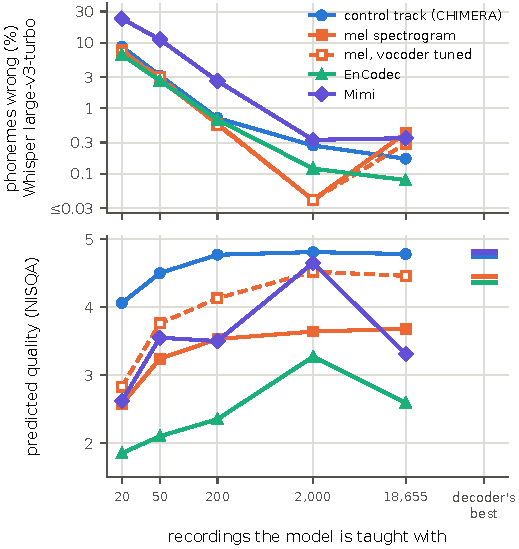
\includegraphics[width=\columnwidth]{fig_control_en.pdf}
\caption{The same model writing four latents, on the 100 test sentences. Top: what Whisper
misreads. Bottom: predicted quality; the bars on the right are each decoder at its best (a
recording through the latent and back; for the control track, encoder I's renders). Dashed:
the spectrogram's vocoder tuned on what the model writes.}
\label{fig:control}
\end{figure}

\begin{table}[t]
\centering\footnotesize\setlength{\tabcolsep}{3pt}
\caption{The control on the 100 test sentences, by the number of recordings the model is taught
with. Best: the decoder's, as in Fig.~\ref{fig:control} (for the tuned vocoder, the one tuned
with all the recordings, on real spectrograms). Held-out: tuned on spectrograms written by
models that did not learn from the recording. $^\dagger$The model of \S\ref{sec:tts}, with
its stand-in loss.}
\label{tab:control}
\begin{tabular}{@{}lrrrrrr@{}}
\toprule
& 20 & 50 & 200 & 2,000 & 18,655 & Best\\
\midrule
\multicolumn{7}{@{}l}{\emph{Whisper large-v3-turbo, phonemes wrong (\%)}}\\
Control track & 8.8 & 3.2 & 0.7 & 0.3 & 0.2$^\dagger$ & 0.1\\
Mel spectrogram & 7.7 & 2.8 & 0.6 & 0.0 & 0.4 & 0.1\\
\quad vocoder tuned & 7.2 & 3.0 & 0.6 & 0.0 & 0.3 & 0.1\\
\quad tuned, held-out & 8.2 & 3.4 & 0.8 & 0.0 & -- & --\\
EnCodec & 6.6 & 2.6 & 0.7 & 0.1 & 0.1 & 0.1\\
Mimi & 23.4 & 11.2 & 2.6 & 0.3 & 0.3 & 0.1\\
\multicolumn{7}{@{}l}{\emph{NISQA}}\\
Control track & 4.06 & 4.50 & 4.77 & 4.81 & 4.78$^\dagger$ & 4.75\\
Mel spectrogram & 2.57 & 3.24 & 3.53 & 3.64 & 3.68 & 4.45\\
\quad vocoder tuned & 2.83 & 3.76 & 4.13 & 4.52 & 4.46 & 4.62\\
\quad tuned, held-out & 3.18 & 3.64 & 3.92 & 4.30 & -- & --\\
EnCodec & 1.85 & 2.10 & 2.35 & 3.27 & 2.59 & 4.36\\
Mimi & 2.62 & 3.55 & 3.50 & 4.65 & 3.31 & 4.81\\
\bottomrule
\end{tabular}
\end{table}

\textbf{The words need little data, whatever the latent.} On the test sentences the spectrogram
and EnCodec are read as well as the control track at every size (Fig.~\ref{fig:control},
Table~\ref{tab:control}): with 200 sentences 0.6\%, 0.7\% and 0.7\% of the phonemes are wrong,
with 20 sentences 7.7\%, 6.6\% and 8.8\%. Only Mimi's wide, slow latent needs more. So the small
appetite for data of \S\ref{sec:tts} is the model's (phonemes and their accent in, durations
given, nothing autoregressive), not the control track's. Nor is the track easier to predict than
a spectrogram: on held-out sentences the model's error is the same share of a value's spread for
both (0.17 with 2,000 sentences), and far larger for the two codecs (0.46 and 0.47).

\textbf{What differs is the sound.} The simulator's renders keep a predicted quality of 4.1 to
4.8 at every size. With the decoders as they are, the spectrogram's are at 2.6 to 3.7 where its vocoder gives 4.45 for a real spectrogram, EnCodec's at 1.9 to 3.3 (4.36) and Mimi's at 2.6 to 4.7 (4.81). An error of the same relative size costs the
vocoder a point and the simulator nothing: a blurred spectrogram is not the spectrogram of a
voice, while a blurred articulation is still an articulation. More data alone does not
close the gap: with all 18,655 sentences the spectrogram's renders are at 3.68, EnCodec's at 2.59
and Mimi's at 3.31, though all are then read almost without error. Nor is the codecs' quality
monotone in the data: with 2,000 sentences Mimi's renders reach 4.65 and EnCodec's 3.27, both
higher than with all. A model that can no longer memorize averages. Its predictions keep 0.95
of the control track's frame-to-frame movement and 0.78 of the spectrogram's; of EnCodec's they
keep 0.61 with 2,000 sentences and 0.49 with all. The track has little detail of the kind that
regression loses. (Every cell is one training run; how much of the codecs' ups and downs is the
run we cannot say.)

\textbf{The vocoder tuned on what the model writes.} A vocoder has learned from the
spectrograms of recordings, and the usual remedy for what it makes of a model's is to tune it
on those~\cite{tacotron2,hifigan}: the spectrograms the model writes for the recordings it
was taught with, given each recording's durations and pitch, with the recording as the target.
We did this for every size, with those recordings and no others. UnivNet is trained on as it
was trained, with its own loss and against its own discriminators, which are in its authors'
checkpoint: 16 stretches of 0.68\,s a step, 1,500 to 15,000 steps by size. The discriminators
are needed. Tuned on the spectral error alone, the renders of validation sentences fell from
3.6 to 2.7; against new discriminators taught for 10,000 steps, to 1.4. The vocoder kept is the
one NISQA rates highest on validation sentences. Nothing else here is chosen by NISQA, so the
choice favours the control (the vocoder of the last step gets 4.02 and 4.36 with 200 and 2,000
sentences; with all, the last step is the one kept).

Tuning raises the spectrogram's renders at every size (Table~\ref{tab:control}, dashed in
Fig.~\ref{fig:control}): from 2.57 to 2.83 with 20 sentences, 3.53 to 4.13 with 200, 3.64 to
4.52 with 2,000 and 3.68 to 4.46 with all. What Whisper misreads does not change. With 2,000
sentences and more the tuned renders are about where the recordings are (4.56), a little under
what the tuned vocoder gives for real spectrograms (4.62): given two and a half hours of the
speaker, the remedy works. With less it works less. A variant for little data has each recording's
spectrogram written by a model that did not learn from it (five folds), so that the vocoder
meets spectrograms as blurred as a new sentence's. It helps with 20 sentences (3.18) and not
with more (3.64, 3.92 and 4.30 with 50, 200 and 2,000). Taking the better of the two, the control
track's renders are ahead by 0.9 with 20 sentences, 0.7 with 50, 0.6 with 200 (15 minutes), and
0.3 with 2,000 and with all, most of which is the simulator scoring above the recordings
themselves.

\textbf{Sentences unlike the corpus.} On the twelve sentences from outside the corpus
(\S\ref{sec:tts}) the controls lose more than on the test sentences: with 200 sentences
large-v3-turbo gets 4.0\% (spectrogram) and 3.0\% (EnCodec) wrong against 0.4\% for the control
track. Twelve sentences give wide intervals ([0.8, 9.2], [0.2, 7.5] and [0.0, 1.0]). With the tuned
vocoder the spectrogram's rate is 1.4\% ([0.6, 2.2]).

\textbf{What the control does not say.} The neural decoders give back the speaker, whose voice
their best is; the simulator has a voice of its own (\S\ref{sec:tts}). They also have none of its
sharp bursts (0.1 to 0.3 releases a second, 25\,dB under the speech, as in recordings; the
simulator's 0.5 to 0.6 at 16\,dB). Only the spectrogram's decoder was tuned; a generative model of the latent in place of
regression, the other usual remedy, was not tried. And the quality is one predictor's. NISQA
has a second model, for the naturalness of synthesized speech, and it ranks the two the other
way: 2.7 to 2.9 for the simulator's renders at every size, 3.5 to 3.9 for the spectrogram's
(3.6 to 4.2 with the tuned vocoder) and 4.5 for the recordings. It marks down the voice, not the
model: encoder I's renders of the recordings get 2.7. The quality score is the one that agreed
with listening, in \S\ref{sec:voice} and for the untuned decoders of this section. What tuning the
vocoder gains, about half a point, the listener could not hear with any confidence.

\section{Towards a release}\label{sec:release}

None of the models above can be passed on. Encoder I hears through mHuBERT and is taught against
it, and mHuBERT's weights, some of which sit inside the encoder's, are licensed for non-commercial
use (CC BY-NC-SA 4.0). JVS is for research and may not be redistributed; Hi-Fi-CAPTAIN is
CC BY-NC-SA. This section rebuilds the chain from what may be: TSP (a BSD licence),
Emilia-YODAS~\cite{emilia} (speech from videos under a Creative Commons licence, CC BY 4.0), and
models whose weights are under Apache-2.0 or MIT: wav2vec 2.0 base, XLS-R~\cite{xlsr} and a
HuBERT trained on Japanese~\cite{jtube}.

\textbf{A pair of voices.} Settings fitted to a speaker need the speaker's recordings, and a
text-to-speech demo has none. The decided settings were therefore reduced to two voices. The high
one is the adjusted voice of \S\ref{sec:voice} on the women's average fitted body, with the larger
sinus and the average of the closures chosen by ear (0.18). The low one is the simulator's adult
male with two habits of posture, the epilarynx held narrow (0.78) and the tongue root 0.35\,cm
forward: tried one at a time, these are the two of the men's eleven numbers that bring a render
nearer its speaker for a verification model (0.870 to 0.903 on the test men; all eleven at their
average give 0.899). Which voice a speaker gets goes by sex and not by pitch. A man's median pitch
reaches 196\,Hz in JVS and a woman's starts at 173\,Hz in TSP, and with the body mixed by pitch
the men's renders moved away from the men (0.850 to 0.812). The voice the encoders had been
taught through did a milder version of that: it gave men above 150\,Hz a share of the soft source
fitted for high voices, three of the four test men among them, and their second harmonic came
out 5.6\,dB too weak. With encoder I's tracks the pair leaves the women's renders where the
per-speaker settings had them on average, and brings the men's to where the eleven numbers had
them (what is missing between 1 and 4\,kHz 5--8\,dB, the second harmonic within 1.1\,dB,
similarity 0.900 against 0.917). It cannot tell speakers apart, and is not meant to.

The pair has a dial. One unit of brightness adds 0.18 to the closure's sharpness and, for the low
voice, 0.22 to the epilarynx: the vowels' level between 2.5 and 4\,kHz moves by 3 to 5\,dB either
way and the second harmonic by less than 1\,dB. And the tracks depend little on the body. A
woman's track played by the low voice ten semitones down, or a man's by the high voice nine
semitones up, is read as well as before (3.1 to 3.8\% by large-v3-turbo). The swap also says
where the women's lower scores come from. Played by the high voice, the men's tracks score as the
women's do (phone mismatch 25.8 $\rightarrow$ 31.7\%, NISQA 4.34 $\rightarrow$ 3.59); played by
the low one, the women's score as the men's (31.7 $\rightarrow$ 29.3\%, 3.64 $\rightarrow$ 4.74).
It is the high voice, not the tracks written for women.

\begin{table}[t]
\centering\footnotesize\setlength{\tabcolsep}{2.6pt}
\caption{Encoders towards a release, on the tests of Table~\ref{tab:japanese}: Whisper
large-v3-turbo errors (\%) and phone mismatch (\%). All but the first row are played by the pair
of voices. Each row changes one thing in the row above it; J and J2 are taught with nothing
but what may be passed on.}
\label{tab:release}
\begin{tabular}{@{}lrrrrrr@{}}
\toprule
& \multicolumn{2}{c}{JVS} & \multicolumn{2}{c}{HFC+JSUT} & \multicolumn{2}{c}{TSP (en)}\\
& err. & phone & err. & phone & err. & phone\\
\midrule
I (its own voice) & 3.4 & 29.3 & 0.4 & 27.3 & 3.2 & 9.4\\
I, played by the pair & 3.4 & 28.8 & 0.5 & 27.6 & 4.2 & 9.7\\
I$'$ (taught by the pair) & 3.6 & 28.0 & 0.5 & 27.2 & 4.1 & 10.1\\
J0 (XLS-R listens) & 5.0 & 32.8 & 1.6 & 31.6 & 7.0 & 12.7\\
J (Emilia for JVS) & 4.9 & 31.5 & 1.2 & 30.7 & 5.0 & 10.6\\
J2 (a HuBERT listens) & 3.6 & 28.1 & 0.5 & 27.5 & 4.6 & 10.5\\
\bottomrule
\end{tabular}
\end{table}

\textbf{Encoders.} Compared as in \S\ref{sec:encoder}, XLS-R's layer 16 hears a Japanese render as
further from its recording than another speaker is, as mHuBERT's layer 8 does ($d'$ 0.97 against
1.32), and an English one too (0.33 against $-0.05$); it became the listener, and wav2vec 2.0
base the front end. Emilia-YODAS does not say a speaker's sex, which picks the voice. Where the
pitch leaves no doubt (a median under 135\,Hz or over 235\,Hz) it decides; a speaker between is
of the sex whose speakers' mean verification vector is nearer, which is right for 90 to 95\% of
such speakers in JVS and TSP. Three encoders separate what each change costs
(Table~\ref{tab:release}). Teaching the encoder through the pair of voices (I$'$) gains little: the
phone mismatch on JVS falls from 28.8 to 28.0\%, and English is a little worse. The models that
may be used cost most: with XLS-R and wav2vec 2.0 base in mHuBERT's place (J0) the mismatch is
32.8\% on JVS and Whisper's error 5.0\% instead of 3.6\%. The recordings cost nothing. With
Emilia-YODAS in JVS's place (J: 300 speakers of each language, six clips each, about six hours)
every test improves, JVS's own included, although J never heard a JVS recording; it has 600
speakers where J0 had 86. On balance J is 3.5 points behind I$'$ in Japanese phone mismatch and
about one point in Whisper's error, and within half a point in English, at the same NISQA.
The loss is the listener's, and another listener undoes it. Of three more encoders on J0's
recordings, the one taught against a HuBERT trained on Japanese alone (hubert-base-jtube~\cite{jtube},
MIT, layer 8) has J0's phone mismatch less 1.8 points and Whisper's error back at I$'$'s, in
English as well as in Japanese (3.3\% on JVS, 5.3\% on TSP; XLS-R as the front end, or its
layer 12 as the listener, gain half as much). With that listener and Emilia-YODAS (J2), an
encoder taught with nothing but what may be passed on is level with I$'$ on every test.

\textbf{Text-to-speech.} The model of \S\ref{sec:tts} was taught again with recordings that may
be passed on, from two corpora and in two shapes. Emilia-YODAS's Japanese is people talking,
written down by a recogniser, and mostly men (about 100 of 800 speakers were placed as women).
Common Voice~\cite{commonvoice} is volunteers reading sentences (CC0), as many women as men,
each in whatever room they had. The model either has a vector for each speaker, as before, or is
told two numbers of a speaker instead: the share of the high voice and the pace. A voice nobody
recorded is then a position of a dial. Three things were learnt (errors are Whisper
large-v3-turbo's, on JVS's test sentences at the recordings' pace). First, a model inherits how
well the encoder copied its corpus. Rendered from J's tracks, Common Voice's recordings are read
with 13.9\% of the phonemes wrong and Emilia-YODAS's with 7.7\% (the recordings themselves: 3.2\%
and 4.0\%), and a model taught with J's tracks of Common Voice gets 6.6 to 15.7\% wrong,
depending on the speaker it speaks as; from J2's tracks the two corpora are read with 7.0\% and
5.0\%. Second, the model that is told the voice reads better than the one with speakers' vectors:
5.4\% in the low voice and 4.1\% in the high one against 11.7\% and 5.7\%, on the same tracks. A
vector learnt from a dozen clips keeps what was wrong with them. Third, with J2's tracks the
dial's model comes level with the recordings: 2.4\% in the low voice when taught with
Emilia-YODAS and 2.8\% in the high voice when taught with Common Voice, where the recordings have
2.5\% and the model taught with JVS 2.3\%. Each corpus is the better one for the voice it has
more clean examples of. A model that is told the voice has no speakers to keep apart, so the two
corpora can be put together (15,279 recordings, 22 hours, about 1,400 speakers). That model gets
3.0\% wrong in the low voice and 2.9\% in the high one: a little behind the better corpus in
each voice, well ahead of the worse (3.6\% and 4.8\%), and the only one whose body can be set
between the two voices. It is the release's Japanese model. Two things had to be set right on
the way. People talking are a third faster than people reading, so the pace is given, and the
listener found the recordings' pace right. And the aligner needs forty epochs with either corpus
where read studio speech needed twelve. The combined model has not been heard yet.

\textbf{English.} The same model was taught for English with the clean hundred hours of
LibriTTS-R~\cite{librittsr} (7,534 sentences of 240 readers, 12.9 hours). Its text is read by
CHIMERA's own English front end, the CMU dictionary with letter-to-sound rules, which is called
as the engine has it. On the 240 test sentences of TSP the model gets 1.9\% of the phonemes
wrong in the low voice and 3.1\% in the high one, where the recordings have 1.6\%.

\textbf{What is published.} A model is published as its weights and a description beside them
that names no speaker of the recordings: speaking in a voice that is told needs only what the
men and the women had at the median (pitch, pace, the pitch's spread). The published model
writes the tracks the trained one wrote.

\textbf{In the browser.} The engine with the track player around it compiles to WebAssembly
(667\,kB) and renders the same samples as the Python module, at more than five times real time
on one core. A page asks a server for a sentence's control track (some tens of kilobytes of
numbers, written in 0.15\,s on two cores) and makes the sound itself, so the pitch and the
brightness can be turned while the voice speaks. The page is remade after CHIMERA's Speak
screen: it draws the midsagittal section in the posture of the frame now sounding, from the
geometry the engine computes its tube from, beside the tube's areas and all 21 channels of the
track. A test drives it in a headless Chrome: with the pitch dial at 120\,Hz the sound that
comes out of the audio thread has a median pitch of 143\,Hz, and of 235\,Hz after the dial is
turned to 240\,Hz in the middle of the sentence.

\section{Discussion}\label{sec:discussion}
\textbf{What mattered.} \emph{Teach through the voice.} Copying tracks averages over ways to
say the same thing; asking that the track sound right, through a crude model of the simulator,
took the encoder from 19.5\% to 6.5\% word errors and made the search unnecessary. \emph{The
listener decides what is learned.} An English listener did not hear Japanese errors, and
distance to it kept falling while the judges did not move. \emph{Listening found what the measures
missed.} Each artifact of \S\ref{sec:voice} was first heard, then located by ear, and only then
measured, twice with a measure that looked in the wrong place; and a quality predictor optimized
on its own found loopholes. \emph{The words are cheap; the sound is
where the decoder counts.} A plain non-autoregressive model needs a hundredth of the data it
was given to be understood, and learns a hundred speakers from 35 seconds of each. The control
shows that this is not the control track's merit: a spectrogram is learned as fast. What the
physical decoder adds is that the little-taught model still sounds like clean speech. A neural
vocoder gets there too once it is tuned on the model's output, but it needs hours of the
speaker for that; with minutes its sound stays behind.

\textbf{Limitations.} The codec carries what is said, its timing and its pitch, and little of who
says it: told a speaker's sex and median pitch, the voice gives renders that a verification
model cannot tell apart within a sex, and with the body, the glottis and the posture fitted to each speaker it finds
the speaker among eight for 57.0\% of them and among a hundred for 14.2\%
(\S\ref{sec:tts}).
The timbre is still the simulator's, and the women's voices, whose vowels are weaker than the
recordings' between 1.6 and 5.5\,kHz, sound less real to the listener than the men's. The bursts
of stops are sharper than a speaker's, more so in the text-to-speech model's renders (0.61 per
second, 15.4\,dB under the speech, against the encoder's 0.54 and 16.3\,dB and the recordings' 0.27
and 25.8\,dB). The mid-vowel timbre of Japanese /e/ is still off. Scores come from ASR and one
quality predictor, with one training run per model, and the listening is one person's. In the
control only the spectrogram's decoder was tuned: EnCodec's and Mimi's were used as they are,
and a generative model of the latent in place of regression was not tried. NISQA's model of
naturalness rates the simulator's voice below the neural decoders' renders
(\S\ref{sec:control}). Accent comes from
Open JTalk's estimate and is wrong where it is.

\section{Conclusion}
A physical model of the voice can be the decoder of a speech codec without being differentiable
or modified: an encoder taught through a learned stand-in writes its control track from a
recording in one pass, and the renders are understood about as well as the recordings. Errors in
this latent come out as poor articulation. The simulator's own artifacts could be traced and
removed through its settings because every part of it means something. And the latent can be
written from text: a small model matches the encoder, fifteen minutes of one speaker are enough
for it to be understood, and with a hundred speakers it reads unseen sentences as intelligibly
as their recordings. That little data suffices is the model's doing, as a control with a
spectrogram and two neural codecs shows. What the physical decoder gives is that the result
sounds like clean speech even when the data is minutes: a neural vocoder tuned on the model's
output needs hours of the speaker to do the same.

\section*{Acknowledgments}
We thank Jameson Hodge for CHIMERA, and the authors of the TSP speech database, JVS, JSUT,
Hi-Fi-CAPTAIN, wav2vec\,2.0, mHuBERT-147, Whisper, NISQA and Open JTalk.

\begin{thebibliography}{99}\footnotesize
\setlength{\itemsep}{0pt}
\bibitem{encodec} A.~Défossez, J.~Copet, G.~Synnaeve, Y.~Adi. High fidelity neural audio
compression. \emph{TMLR}, 2023.
\bibitem{moshi} A.~Défossez et al. Moshi: a speech-text foundation model for real-time dialogue.
arXiv:2410.00037, 2024.
\bibitem{pocketja} Claude, T.~Mori. Pocket TTS learns Japanese: Training data and distillation for
a drop-in 100M-parameter model. Technical report, 2026.
\bibitem{sparc} C.~J.~Cho, P.~Wu, T.~S.~Prabhune, D.~Agarwal, G.~K.~Anumanchipalli. Coding speech
through vocal tract kinematics. arXiv:2406.12998, 2024.
\bibitem{arti6} J.~Lee et al. ARTI-6: Towards six-dimensional articulatory speech encoding.
arXiv:2509.21447, 2025.
\bibitem{difftlm} E.~M.~Chen, J.~W.~Lee, V.~Sitzmann. Reconstructing the vocal tract with
differentiable acoustic simulation. arXiv:2609.36737, 2026.
\bibitem{vtl} P.~Birkholz. VocalTractLab. \url{https://www.vocaltractlab.de}.
\bibitem{chimera} J.~Hodge. CHIMERA: a physical-modeling voice synthesizer.
\url{https://github.com/jamesondh/chimera-vocal-synth}, 2026.
\bibitem{tsp} P.~Kabal. TSP speech database. Technical report, McGill University, 2002.
\bibitem{jvs} S.~Takamichi et al. JVS corpus: free Japanese multi-speaker voice corpus.
arXiv:1908.06248, 2019.
\bibitem{hificaptain} NICT. Hi-Fi-CAPTAIN corpus.
\url{https://ast-astrec.nict.go.jp/en/release/hi-fi-captain/}.
\bibitem{jsut} R.~Sonobe, S.~Takamichi, H.~Saruwatari. JSUT corpus: free large-scale Japanese
speech corpus for end-to-end speech synthesis. arXiv:1711.00354, 2017.
\bibitem{whisper} A.~Radford et al. Robust speech recognition via large-scale weak supervision.
\emph{ICML}, 2023.
\bibitem{openjtalk} Open JTalk. \url{https://open-jtalk.sourceforge.net}.
\bibitem{xlsrphone} Q.~Xu, A.~Baevski, M.~Auli. Simple and effective zero-shot cross-lingual
phoneme recognition. \emph{Interspeech}, 2022.
\bibitem{nisqa} G.~Mittag, B.~Naderi, A.~Chehadi, S.~Möller. NISQA: A deep CNN-self-attention
model for multidimensional speech quality prediction with crowdsourced datasets.
\emph{Interspeech}, 2021.
\bibitem{praat} P.~Boersma. Accurate short-term analysis of the fundamental frequency and the
harmonics-to-noise ratio of a sampled sound. \emph{IFA Proceedings} 17, 1993.
\bibitem{distal} M.~I.~Jordan, D.~E.~Rumelhart. Forward models: Supervised learning with a distal
teacher. \emph{Cognitive Science} 16(3), 1992.
\bibitem{wav2vec2} A.~Baevski, Y.~Zhou, A.~Mohamed, M.~Auli. wav2vec 2.0: A framework for
self-supervised learning of speech representations. \emph{NeurIPS}, 2020.
\bibitem{mhubert} M.~Zanon~Boito, V.~Iyer, N.~Lagos, L.~Besacier, I.~Calapodescu. mHuBERT-147: A
compact multilingual HuBERT model. \emph{Interspeech}, 2024.
\bibitem{univnet} W.~Jang, D.~Lim, J.~Yoon, B.~Kim, J.~Kim. UnivNet: A neural vocoder with
multi-resolution spectrogram discriminators for high-fidelity waveform generation.
\emph{Interspeech}, 2021.
\bibitem{tacotron2} J.~Shen et al. Natural TTS synthesis by conditioning WaveNet on mel
spectrogram predictions. \emph{ICASSP}, 2018.
\bibitem{hifigan} J.~Kong, J.~Kim, J.~Bae. HiFi-GAN: Generative adversarial networks for
efficient and high fidelity speech synthesis. \emph{NeurIPS}, 2020.
\bibitem{unispeechsat} S.~Chen et al. UniSpeech-SAT: Universal speech representation learning
with speaker aware pre-training. \emph{ICASSP}, 2022.
\bibitem{wavlm} S.~Chen et al. WavLM: Large-scale self-supervised pre-training for full stack
speech processing. \emph{IEEE JSTSP} 16(6), 2022.
\bibitem{fastspeech2} Y.~Ren et al. FastSpeech 2: Fast and high-quality end-to-end text to speech.
\emph{ICLR}, 2021.
\bibitem{ota} R.~Badlani, A.~Łańcucki, K.~J.~Shih, R.~Valle, W.~Ping, B.~Catanzaro. One TTS
alignment to rule them all. \emph{ICASSP}, 2022.
\bibitem{emilia} H.~He et al. Emilia: A large-scale, extensive, multilingual, and diverse dataset
for speech generation. arXiv:2501.15907, 2025.
\bibitem{xlsr} A.~Babu et al. XLS-R: Self-supervised cross-lingual speech representation learning
at scale. Interspeech, 2022.
\bibitem{jtube} sarulab-speech. hubert-base-jtube: a HuBERT model trained on JTubeSpeech.
\url{https://huggingface.co/sarulab-speech/hubert-base-jtube}.
\bibitem{commonvoice} R.~Ardila et al. Common Voice: A massively-multilingual speech corpus. LREC, 2020.
\bibitem{librittsr} Y.~Koizumi et al. LibriTTS-R: A restored multi-speaker text-to-speech corpus. Interspeech, 2023.
\end{thebibliography}
\end{document}
